% SOURCE: ../../edit-harness/results/frame_a/cells/cell_*_real_MIX_A_*.json
% !TEX encoding = UTF-8 Unicode
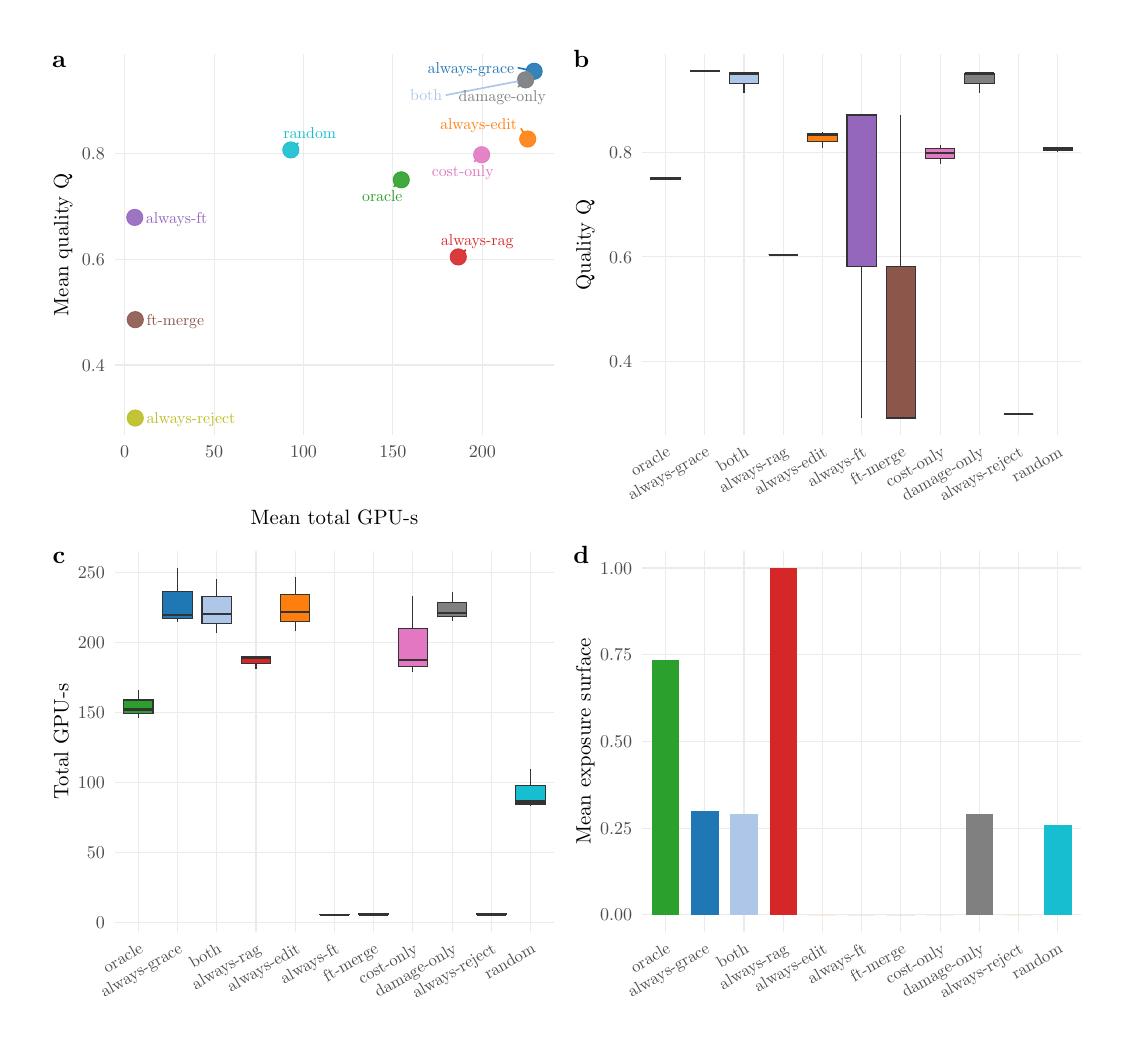
\begin{tikzpicture}[x=1pt,y=1pt]
\definecolor{fillColor}{RGB}{255,255,255}
\path[use as bounding box,fill=fillColor,fill opacity=0.00] (0,0) rectangle (390.26,361.35);
\begin{scope}
\path[clip] (  0.00,  0.00) rectangle (390.26,361.35);
\definecolor{drawColor}{RGB}{255,255,255}
\definecolor{fillColor}{RGB}{255,255,255}

\path[draw=drawColor,line width= 0.6pt,line join=round,line cap=round,fill=fillColor] (  0.00,  0.00) rectangle (390.26,361.35);
\end{scope}
\begin{scope}
\path[clip] (  5.50,176.36) rectangle (194.23,355.85);
\definecolor{fillColor}{RGB}{255,255,255}

\path[fill=fillColor] (  5.50,176.36) rectangle (194.23,355.85);
\end{scope}
\begin{scope}
\path[clip] (194.23,176.36) rectangle (384.76,355.85);
\definecolor{fillColor}{RGB}{255,255,255}

\path[fill=fillColor] (194.23,176.36) rectangle (384.76,355.85);
\end{scope}
\begin{scope}
\path[clip] (  5.50,  5.50) rectangle (194.23,176.36);
\definecolor{fillColor}{RGB}{255,255,255}

\path[fill=fillColor] (  5.50,  5.50) rectangle (194.23,176.36);
\end{scope}
\begin{scope}
\path[clip] (194.23,  5.50) rectangle (384.76,176.36);
\definecolor{fillColor}{RGB}{255,255,255}

\path[fill=fillColor] (194.23,  5.50) rectangle (384.76,176.36);
\end{scope}
\begin{scope}
\path[clip] ( 31.47,214.03) rectangle (190.23,351.85);
\definecolor{drawColor}{gray}{0.92}

\path[draw=drawColor,line width= 0.4pt,line join=round] ( 31.47,239.44) --
	(190.23,239.44);

\path[draw=drawColor,line width= 0.4pt,line join=round] ( 31.47,277.73) --
	(190.23,277.73);

\path[draw=drawColor,line width= 0.4pt,line join=round] ( 31.47,316.02) --
	(190.23,316.02);

\path[draw=drawColor,line width= 0.4pt,line join=round] ( 35.07,214.03) --
	( 35.07,351.85);

\path[draw=drawColor,line width= 0.4pt,line join=round] ( 67.37,214.03) --
	( 67.37,351.85);

\path[draw=drawColor,line width= 0.4pt,line join=round] ( 99.67,214.03) --
	( 99.67,351.85);

\path[draw=drawColor,line width= 0.4pt,line join=round] (131.97,214.03) --
	(131.97,351.85);

\path[draw=drawColor,line width= 0.4pt,line join=round] (164.27,214.03) --
	(164.27,351.85);
\definecolor{drawColor}{RGB}{44,160,44}
\definecolor{fillColor}{RGB}{44,160,44}

\path[draw=drawColor,draw opacity=0.90,line width= 0.3pt,line join=round,line cap=round,fill=fillColor,fill opacity=0.90] (135.00,306.37) circle (  2.94);
\definecolor{drawColor}{RGB}{31,119,180}
\definecolor{fillColor}{RGB}{31,119,180}

\path[draw=drawColor,draw opacity=0.90,line width= 0.3pt,line join=round,line cap=round,fill=fillColor,fill opacity=0.90] (183.01,345.59) circle (  2.94);
\definecolor{drawColor}{RGB}{174,199,232}
\definecolor{fillColor}{RGB}{174,199,232}

\path[draw=drawColor,draw opacity=0.90,line width= 0.3pt,line join=round,line cap=round,fill=fillColor,fill opacity=0.90] (179.82,342.50) circle (  2.94);
\definecolor{drawColor}{RGB}{214,39,40}
\definecolor{fillColor}{RGB}{214,39,40}

\path[draw=drawColor,draw opacity=0.90,line width= 0.3pt,line join=round,line cap=round,fill=fillColor,fill opacity=0.90] (155.60,278.50) circle (  2.94);
\definecolor{drawColor}{RGB}{255,127,14}
\definecolor{fillColor}{RGB}{255,127,14}

\path[draw=drawColor,draw opacity=0.90,line width= 0.3pt,line join=round,line cap=round,fill=fillColor,fill opacity=0.90] (180.69,321.11) circle (  2.94);
\definecolor{drawColor}{RGB}{148,103,189}
\definecolor{fillColor}{RGB}{148,103,189}

\path[draw=drawColor,draw opacity=0.90,line width= 0.3pt,line join=round,line cap=round,fill=fillColor,fill opacity=0.90] ( 38.69,292.78) circle (  2.94);
\definecolor{drawColor}{RGB}{140,86,75}
\definecolor{fillColor}{RGB}{140,86,75}

\path[draw=drawColor,draw opacity=0.90,line width= 0.3pt,line join=round,line cap=round,fill=fillColor,fill opacity=0.90] ( 38.88,255.84) circle (  2.94);
\definecolor{drawColor}{RGB}{227,119,194}
\definecolor{fillColor}{RGB}{227,119,194}

\path[draw=drawColor,draw opacity=0.90,line width= 0.3pt,line join=round,line cap=round,fill=fillColor,fill opacity=0.90] (164.05,315.42) circle (  2.94);
\definecolor{drawColor}{RGB}{127,127,127}
\definecolor{fillColor}{RGB}{127,127,127}

\path[draw=drawColor,draw opacity=0.90,line width= 0.3pt,line join=round,line cap=round,fill=fillColor,fill opacity=0.90] (179.96,342.50) circle (  2.94);
\definecolor{drawColor}{RGB}{188,189,34}
\definecolor{fillColor}{RGB}{188,189,34}

\path[draw=drawColor,draw opacity=0.90,line width= 0.3pt,line join=round,line cap=round,fill=fillColor,fill opacity=0.90] ( 38.88,220.29) circle (  2.94);
\definecolor{drawColor}{RGB}{23,190,207}
\definecolor{fillColor}{RGB}{23,190,207}

\path[draw=drawColor,draw opacity=0.90,line width= 0.3pt,line join=round,line cap=round,fill=fillColor,fill opacity=0.90] ( 95.08,317.16) circle (  2.94);
\definecolor{drawColor}{RGB}{44,160,44}

\path[draw=drawColor,line width= 0.6pt,line join=round,line cap=round] (132.37,303.91) -- (132.90,304.40);
\definecolor{drawColor}{RGB}{31,119,180}

\path[draw=drawColor,line width= 0.6pt,line join=round,line cap=round] (177.24,346.84) -- (180.20,346.20);
\definecolor{drawColor}{RGB}{174,199,232}

\path[draw=drawColor,line width= 0.6pt,line join=round,line cap=round] (151.25,337.00) -- (177.00,341.95);
\definecolor{drawColor}{RGB}{214,39,40}

\path[draw=drawColor,line width= 0.6pt,line join=round,line cap=round] (158.23,280.98) -- (157.69,280.47);
\definecolor{drawColor}{RGB}{255,127,14}

\path[draw=drawColor,line width= 0.6pt,line join=round,line cap=round] (178.29,324.83) -- (179.13,323.53);
\definecolor{drawColor}{RGB}{227,119,194}

\path[draw=drawColor,line width= 0.6pt,line join=round,line cap=round] (161.42,312.95) -- (161.95,313.45);
\definecolor{drawColor}{gray}{0.50}

\path[draw=drawColor,line width= 0.6pt,line join=round,line cap=round] (177.24,340.00) -- (177.84,340.55);
\definecolor{drawColor}{RGB}{23,190,207}

\path[draw=drawColor,line width= 0.6pt,line join=round,line cap=round] ( 97.72,319.64) -- ( 97.18,319.13);
\definecolor{drawColor}{RGB}{44,160,44}

\node[text=drawColor,anchor=base,inner sep=0pt, outer sep=0pt, scale=  0.57] at (128.15,298.48) {oracle};
\definecolor{drawColor}{RGB}{31,119,180}

\node[text=drawColor,anchor=base,inner sep=0pt, outer sep=0pt, scale=  0.57] at (160.14,344.92) {always-grace};
\definecolor{drawColor}{RGB}{174,199,232}

\node[text=drawColor,anchor=base,inner sep=0pt, outer sep=0pt, scale=  0.57] at (143.98,334.97) {both};
\definecolor{drawColor}{RGB}{214,39,40}

\node[text=drawColor,anchor=base,inner sep=0pt, outer sep=0pt, scale=  0.57] at (162.44,282.48) {always-rag};
\definecolor{drawColor}{RGB}{255,127,14}

\node[text=drawColor,anchor=base,inner sep=0pt, outer sep=0pt, scale=  0.57] at (162.94,324.62) {always-edit};
\definecolor{drawColor}{RGB}{148,103,189}

\node[text=drawColor,anchor=base,inner sep=0pt, outer sep=0pt, scale=  0.57] at ( 53.83,290.73) {always-ft};
\definecolor{drawColor}{RGB}{140,86,75}

\node[text=drawColor,anchor=base,inner sep=0pt, outer sep=0pt, scale=  0.57] at ( 53.37,253.91) {ft-merge};
\definecolor{drawColor}{RGB}{227,119,194}

\node[text=drawColor,anchor=base,inner sep=0pt, outer sep=0pt, scale=  0.57] at (157.22,307.53) {cost-only};
\definecolor{drawColor}{gray}{0.50}

\node[text=drawColor,anchor=base,inner sep=0pt, outer sep=0pt, scale=  0.57] at (171.49,334.58) {damage-only};
\definecolor{drawColor}{RGB}{188,189,34}

\node[text=drawColor,anchor=base,inner sep=0pt, outer sep=0pt, scale=  0.57] at ( 58.97,218.16) {always-reject};
\definecolor{drawColor}{RGB}{23,190,207}

\node[text=drawColor,anchor=base,inner sep=0pt, outer sep=0pt, scale=  0.57] at (101.92,321.14) {random};
\end{scope}
\begin{scope}
\path[clip] (  0.00,  0.00) rectangle (390.26,361.35);
\definecolor{drawColor}{gray}{0.30}

\node[text=drawColor,anchor=base east,inner sep=0pt, outer sep=0pt, scale=  0.65] at ( 27.87,237.20) {0.4};

\node[text=drawColor,anchor=base east,inner sep=0pt, outer sep=0pt, scale=  0.65] at ( 27.87,275.49) {0.6};

\node[text=drawColor,anchor=base east,inner sep=0pt, outer sep=0pt, scale=  0.65] at ( 27.87,313.79) {0.8};
\end{scope}
\begin{scope}
\path[clip] (  0.00,  0.00) rectangle (390.26,361.35);
\definecolor{drawColor}{gray}{0.30}

\node[text=drawColor,anchor=base,inner sep=0pt, outer sep=0pt, scale=  0.65] at ( 35.07,205.95) {0};

\node[text=drawColor,anchor=base,inner sep=0pt, outer sep=0pt, scale=  0.65] at ( 67.37,205.95) {50};

\node[text=drawColor,anchor=base,inner sep=0pt, outer sep=0pt, scale=  0.65] at ( 99.67,205.95) {100};

\node[text=drawColor,anchor=base,inner sep=0pt, outer sep=0pt, scale=  0.65] at (131.97,205.95) {150};

\node[text=drawColor,anchor=base,inner sep=0pt, outer sep=0pt, scale=  0.65] at (164.27,205.95) {200};
\end{scope}
\begin{scope}
\path[clip] (  0.00,  0.00) rectangle (390.26,361.35);
\definecolor{drawColor}{RGB}{0,0,0}

\node[text=drawColor,anchor=base,inner sep=0pt, outer sep=0pt, scale=  0.75] at (110.85,181.82) {Mean total GPU-s};
\end{scope}
\begin{scope}
\path[clip] (  0.00,  0.00) rectangle (390.26,361.35);
\definecolor{drawColor}{RGB}{0,0,0}

\node[text=drawColor,rotate= 90.00,anchor=base,inner sep=0pt, outer sep=0pt, scale=  0.75] at ( 14.67,282.94) {Mean quality Q};
\end{scope}
\begin{scope}
\path[clip] (  0.00,  0.00) rectangle (390.26,361.35);
\definecolor{drawColor}{RGB}{0,0,0}

\node[text=drawColor,anchor=base,inner sep=0pt, outer sep=0pt, scale=  0.90] at ( 11.31,347.03) {\bfseries a};
\end{scope}
\begin{scope}
\path[clip] (222.00,214.03) rectangle (380.76,351.85);
\definecolor{drawColor}{gray}{0.92}

\path[draw=drawColor,line width= 0.4pt,line join=round] (222.00,240.64) --
	(380.76,240.64);

\path[draw=drawColor,line width= 0.4pt,line join=round] (222.00,278.50) --
	(380.76,278.50);

\path[draw=drawColor,line width= 0.4pt,line join=round] (222.00,316.36) --
	(380.76,316.36);

\path[draw=drawColor,line width= 0.4pt,line join=round] (230.51,214.03) --
	(230.51,351.85);

\path[draw=drawColor,line width= 0.4pt,line join=round] (244.68,214.03) --
	(244.68,351.85);

\path[draw=drawColor,line width= 0.4pt,line join=round] (258.86,214.03) --
	(258.86,351.85);

\path[draw=drawColor,line width= 0.4pt,line join=round] (273.03,214.03) --
	(273.03,351.85);

\path[draw=drawColor,line width= 0.4pt,line join=round] (287.21,214.03) --
	(287.21,351.85);

\path[draw=drawColor,line width= 0.4pt,line join=round] (301.38,214.03) --
	(301.38,351.85);

\path[draw=drawColor,line width= 0.4pt,line join=round] (315.55,214.03) --
	(315.55,351.85);

\path[draw=drawColor,line width= 0.4pt,line join=round] (329.73,214.03) --
	(329.73,351.85);

\path[draw=drawColor,line width= 0.4pt,line join=round] (343.90,214.03) --
	(343.90,351.85);

\path[draw=drawColor,line width= 0.4pt,line join=round] (358.08,214.03) --
	(358.08,351.85);

\path[draw=drawColor,line width= 0.4pt,line join=round] (372.25,214.03) --
	(372.25,351.85);
\definecolor{drawColor}{gray}{0.20}

\path[draw=drawColor,line width= 0.4pt,line join=round] (230.51,307.04) -- (230.51,307.27);

\path[draw=drawColor,line width= 0.4pt,line join=round] (230.51,306.59) -- (230.51,306.36);
\definecolor{fillColor}{RGB}{44,160,44}

\path[draw=drawColor,line width= 0.4pt,fill=fillColor] (225.19,307.04) --
	(225.19,306.59) --
	(235.82,306.59) --
	(235.82,307.04) --
	(225.19,307.04) --
	cycle;

\path[draw=drawColor,line width= 0.8pt] (225.19,306.82) -- (235.82,306.82);

\path[draw=drawColor,line width= 0.4pt,line join=round] (244.68,345.59) -- (244.68,345.59);

\path[draw=drawColor,line width= 0.4pt,line join=round] (244.68,345.59) -- (244.68,345.59);
\definecolor{fillColor}{RGB}{31,119,180}

\path[draw=drawColor,line width= 0.4pt,fill=fillColor] (239.37,345.59) --
	(239.37,345.59) --
	(250.00,345.59) --
	(250.00,345.59) --
	(239.37,345.59) --
	cycle;

\path[draw=drawColor,line width= 0.8pt] (239.37,345.59) -- (250.00,345.59);

\path[draw=drawColor,line width= 0.4pt,line join=round] (258.86,344.89) -- (258.86,345.00);

\path[draw=drawColor,line width= 0.4pt,line join=round] (258.86,341.30) -- (258.86,337.82);
\definecolor{fillColor}{RGB}{174,199,232}

\path[draw=drawColor,line width= 0.4pt,fill=fillColor] (253.54,344.89) --
	(253.54,341.30) --
	(264.17,341.30) --
	(264.17,344.89) --
	(253.54,344.89) --
	cycle;

\path[draw=drawColor,line width= 0.8pt] (253.54,344.78) -- (264.17,344.78);

\path[draw=drawColor,line width= 0.4pt,line join=round] (273.03,279.26) -- (273.03,279.26);

\path[draw=drawColor,line width= 0.4pt,line join=round] (273.03,279.26) -- (273.03,279.26);
\definecolor{fillColor}{RGB}{214,39,40}

\path[draw=drawColor,line width= 0.4pt,fill=fillColor] (267.72,279.26) --
	(267.72,279.26) --
	(278.35,279.26) --
	(278.35,279.26) --
	(267.72,279.26) --
	cycle;

\path[draw=drawColor,line width= 0.8pt] (267.72,279.26) -- (278.35,279.26);

\path[draw=drawColor,line width= 0.4pt,line join=round] (287.21,323.22) -- (287.21,323.82);

\path[draw=drawColor,line width= 0.4pt,line join=round] (287.21,320.17) -- (287.21,317.73);
\definecolor{fillColor}{RGB}{255,127,14}

\path[draw=drawColor,line width= 0.4pt,fill=fillColor] (281.89,323.22) --
	(281.89,320.17) --
	(292.52,320.17) --
	(292.52,323.22) --
	(281.89,323.22) --
	cycle;

\path[draw=drawColor,line width= 0.8pt] (281.89,322.61) -- (292.52,322.61);

\path[draw=drawColor,line width= 0.4pt,line join=round] (301.38,329.91) -- (301.38,329.91);

\path[draw=drawColor,line width= 0.4pt,line join=round] (301.38,275.10) -- (301.38,220.29);
\definecolor{fillColor}{RGB}{148,103,189}

\path[draw=drawColor,line width= 0.4pt,fill=fillColor] (296.06,329.91) --
	(296.06,275.10) --
	(306.70,275.10) --
	(306.70,329.91) --
	(296.06,329.91) --
	cycle;

\path[draw=drawColor,line width= 0.8pt] (296.06,329.91) -- (306.70,329.91);

\path[draw=drawColor,line width= 0.4pt,line join=round] (315.55,275.13) -- (315.55,329.91);

\path[draw=drawColor,line width= 0.4pt,line join=round] (315.55,220.32) -- (315.55,220.29);
\definecolor{fillColor}{RGB}{140,86,75}

\path[draw=drawColor,line width= 0.4pt,fill=fillColor] (310.24,275.13) --
	(310.24,220.32) --
	(320.87,220.32) --
	(320.87,275.13) --
	(310.24,275.13) --
	cycle;

\path[draw=drawColor,line width= 0.8pt] (310.24,220.34) -- (320.87,220.34);

\path[draw=drawColor,line width= 0.4pt,line join=round] (329.73,317.66) -- (329.73,319.12);

\path[draw=drawColor,line width= 0.4pt,line join=round] (329.73,314.09) -- (329.73,311.97);
\definecolor{fillColor}{RGB}{227,119,194}

\path[draw=drawColor,line width= 0.4pt,fill=fillColor] (324.41,317.66) --
	(324.41,314.09) --
	(335.04,314.09) --
	(335.04,317.66) --
	(324.41,317.66) --
	cycle;

\path[draw=drawColor,line width= 0.8pt] (324.41,316.20) -- (335.04,316.20);

\path[draw=drawColor,line width= 0.4pt,line join=round] (343.90,344.89) -- (343.90,345.00);

\path[draw=drawColor,line width= 0.4pt,line join=round] (343.90,341.30) -- (343.90,337.82);
\definecolor{fillColor}{gray}{0.50}

\path[draw=drawColor,line width= 0.4pt,fill=fillColor] (338.59,344.89) --
	(338.59,341.30) --
	(349.22,341.30) --
	(349.22,344.89) --
	(338.59,344.89) --
	cycle;

\path[draw=drawColor,line width= 0.8pt] (338.59,344.78) -- (349.22,344.78);

\path[draw=drawColor,line width= 0.4pt,line join=round] (358.08,221.71) -- (358.08,221.71);

\path[draw=drawColor,line width= 0.4pt,line join=round] (358.08,221.71) -- (358.08,221.71);
\definecolor{fillColor}{RGB}{188,189,34}

\path[draw=drawColor,line width= 0.4pt,fill=fillColor] (352.76,221.71) --
	(352.76,221.71) --
	(363.39,221.71) --
	(363.39,221.71) --
	(352.76,221.71) --
	cycle;

\path[draw=drawColor,line width= 0.8pt] (352.76,221.71) -- (363.39,221.71);

\path[draw=drawColor,line width= 0.4pt,line join=round] (372.25,318.06) -- (372.25,318.18);

\path[draw=drawColor,line width= 0.4pt,line join=round] (372.25,317.13) -- (372.25,316.32);
\definecolor{fillColor}{RGB}{23,190,207}

\path[draw=drawColor,line width= 0.4pt,fill=fillColor] (366.94,318.06) --
	(366.94,317.13) --
	(377.57,317.13) --
	(377.57,318.06) --
	(366.94,318.06) --
	cycle;

\path[draw=drawColor,line width= 0.8pt] (366.94,317.93) -- (377.57,317.93);
\end{scope}
\begin{scope}
\path[clip] (  0.00,  0.00) rectangle (390.26,361.35);
\definecolor{drawColor}{gray}{0.30}

\node[text=drawColor,anchor=base east,inner sep=0pt, outer sep=0pt, scale=  0.65] at (218.40,238.40) {0.4};

\node[text=drawColor,anchor=base east,inner sep=0pt, outer sep=0pt, scale=  0.65] at (218.40,276.26) {0.6};

\node[text=drawColor,anchor=base east,inner sep=0pt, outer sep=0pt, scale=  0.65] at (218.40,314.12) {0.8};
\end{scope}
\begin{scope}
\path[clip] (  0.00,  0.00) rectangle (390.26,361.35);
\definecolor{drawColor}{gray}{0.30}

\node[text=drawColor,rotate= 30.00,anchor=base east,inner sep=0pt, outer sep=0pt, scale=  0.60] at (232.57,206.85) {oracle};

\node[text=drawColor,rotate= 30.00,anchor=base east,inner sep=0pt, outer sep=0pt, scale=  0.60] at (246.75,206.85) {always-grace};

\node[text=drawColor,rotate= 30.00,anchor=base east,inner sep=0pt, outer sep=0pt, scale=  0.60] at (260.92,206.85) {both};

\node[text=drawColor,rotate= 30.00,anchor=base east,inner sep=0pt, outer sep=0pt, scale=  0.60] at (275.10,206.85) {always-rag};

\node[text=drawColor,rotate= 30.00,anchor=base east,inner sep=0pt, outer sep=0pt, scale=  0.60] at (289.27,206.85) {always-edit};

\node[text=drawColor,rotate= 30.00,anchor=base east,inner sep=0pt, outer sep=0pt, scale=  0.60] at (303.45,206.85) {always-ft};

\node[text=drawColor,rotate= 30.00,anchor=base east,inner sep=0pt, outer sep=0pt, scale=  0.60] at (317.62,206.85) {ft-merge};

\node[text=drawColor,rotate= 30.00,anchor=base east,inner sep=0pt, outer sep=0pt, scale=  0.60] at (331.80,206.85) {cost-only};

\node[text=drawColor,rotate= 30.00,anchor=base east,inner sep=0pt, outer sep=0pt, scale=  0.60] at (345.97,206.85) {damage-only};

\node[text=drawColor,rotate= 30.00,anchor=base east,inner sep=0pt, outer sep=0pt, scale=  0.60] at (360.14,206.85) {always-reject};

\node[text=drawColor,rotate= 30.00,anchor=base east,inner sep=0pt, outer sep=0pt, scale=  0.60] at (374.32,206.85) {random};
\end{scope}
\begin{scope}
\path[clip] (  0.00,  0.00) rectangle (390.26,361.35);
\definecolor{drawColor}{RGB}{0,0,0}

\node[text=drawColor,rotate= 90.00,anchor=base,inner sep=0pt, outer sep=0pt, scale=  0.75] at (203.39,282.94) {Quality Q};
\end{scope}
\begin{scope}
\path[clip] (  0.00,  0.00) rectangle (390.26,361.35);
\definecolor{drawColor}{RGB}{0,0,0}

\node[text=drawColor,anchor=base,inner sep=0pt, outer sep=0pt, scale=  0.90] at (200.05,347.03) {\bfseries b};
\end{scope}
\begin{scope}
\path[clip] ( 31.47, 34.54) rectangle (190.23,172.36);
\definecolor{drawColor}{gray}{0.92}

\path[draw=drawColor,line width= 0.4pt,line join=round] ( 31.47, 38.01) --
	(190.23, 38.01);

\path[draw=drawColor,line width= 0.4pt,line join=round] ( 31.47, 63.31) --
	(190.23, 63.31);

\path[draw=drawColor,line width= 0.4pt,line join=round] ( 31.47, 88.61) --
	(190.23, 88.61);

\path[draw=drawColor,line width= 0.4pt,line join=round] ( 31.47,113.91) --
	(190.23,113.91);

\path[draw=drawColor,line width= 0.4pt,line join=round] ( 31.47,139.21) --
	(190.23,139.21);

\path[draw=drawColor,line width= 0.4pt,line join=round] ( 31.47,164.51) --
	(190.23,164.51);

\path[draw=drawColor,line width= 0.4pt,line join=round] ( 39.98, 34.54) --
	( 39.98,172.36);

\path[draw=drawColor,line width= 0.4pt,line join=round] ( 54.15, 34.54) --
	( 54.15,172.36);

\path[draw=drawColor,line width= 0.4pt,line join=round] ( 68.32, 34.54) --
	( 68.32,172.36);

\path[draw=drawColor,line width= 0.4pt,line join=round] ( 82.50, 34.54) --
	( 82.50,172.36);

\path[draw=drawColor,line width= 0.4pt,line join=round] ( 96.67, 34.54) --
	( 96.67,172.36);

\path[draw=drawColor,line width= 0.4pt,line join=round] (110.85, 34.54) --
	(110.85,172.36);

\path[draw=drawColor,line width= 0.4pt,line join=round] (125.02, 34.54) --
	(125.02,172.36);

\path[draw=drawColor,line width= 0.4pt,line join=round] (139.20, 34.54) --
	(139.20,172.36);

\path[draw=drawColor,line width= 0.4pt,line join=round] (153.37, 34.54) --
	(153.37,172.36);

\path[draw=drawColor,line width= 0.4pt,line join=round] (167.55, 34.54) --
	(167.55,172.36);

\path[draw=drawColor,line width= 0.4pt,line join=round] (181.72, 34.54) --
	(181.72,172.36);
\definecolor{drawColor}{gray}{0.20}

\path[draw=drawColor,line width= 0.4pt,line join=round] ( 39.98,118.41) -- ( 39.98,121.84);

\path[draw=drawColor,line width= 0.4pt,line join=round] ( 39.98,113.50) -- ( 39.98,112.03);
\definecolor{fillColor}{RGB}{44,160,44}

\path[draw=drawColor,line width= 0.4pt,fill=fillColor] ( 34.66,118.41) --
	( 34.66,113.50) --
	( 45.29,113.50) --
	( 45.29,118.41) --
	( 34.66,118.41) --
	cycle;

\path[draw=drawColor,line width= 0.8pt] ( 34.66,114.97) -- ( 45.29,114.97);

\path[draw=drawColor,line width= 0.4pt,line join=round] ( 54.15,157.56) -- ( 54.15,166.10);

\path[draw=drawColor,line width= 0.4pt,line join=round] ( 54.15,147.78) -- ( 54.15,146.55);
\definecolor{fillColor}{RGB}{31,119,180}

\path[draw=drawColor,line width= 0.4pt,fill=fillColor] ( 48.83,157.56) --
	( 48.83,147.78) --
	( 59.47,147.78) --
	( 59.47,157.56) --
	( 48.83,157.56) --
	cycle;

\path[draw=drawColor,line width= 0.8pt] ( 48.83,149.01) -- ( 59.47,149.01);

\path[draw=drawColor,line width= 0.4pt,line join=round] ( 68.32,155.84) -- ( 68.32,162.11);

\path[draw=drawColor,line width= 0.4pt,line join=round] ( 68.32,146.03) -- ( 68.32,142.49);
\definecolor{fillColor}{RGB}{174,199,232}

\path[draw=drawColor,line width= 0.4pt,fill=fillColor] ( 63.01,155.84) --
	( 63.01,146.03) --
	( 73.64,146.03) --
	( 73.64,155.84) --
	( 63.01,155.84) --
	cycle;

\path[draw=drawColor,line width= 0.8pt] ( 63.01,149.57) -- ( 73.64,149.57);

\path[draw=drawColor,line width= 0.4pt,line join=round] ( 82.50,133.85) -- ( 82.50,133.94);

\path[draw=drawColor,line width= 0.4pt,line join=round] ( 82.50,131.65) -- ( 82.50,129.54);
\definecolor{fillColor}{RGB}{214,39,40}

\path[draw=drawColor,line width= 0.4pt,fill=fillColor] ( 77.18,133.85) --
	( 77.18,131.65) --
	( 87.81,131.65) --
	( 87.81,133.85) --
	( 77.18,133.85) --
	cycle;

\path[draw=drawColor,line width= 0.8pt] ( 77.18,133.77) -- ( 87.81,133.77);

\path[draw=drawColor,line width= 0.4pt,line join=round] ( 96.67,156.49) -- ( 96.67,162.72);

\path[draw=drawColor,line width= 0.4pt,line join=round] ( 96.67,146.75) -- ( 96.67,143.25);
\definecolor{fillColor}{RGB}{255,127,14}

\path[draw=drawColor,line width= 0.4pt,fill=fillColor] ( 91.36,156.49) --
	( 91.36,146.75) --
	(101.99,146.75) --
	(101.99,156.49) --
	( 91.36,156.49) --
	cycle;

\path[draw=drawColor,line width= 0.8pt] ( 91.36,150.25) -- (101.99,150.25);

\path[draw=drawColor,line width= 0.4pt,line join=round] (110.85, 40.86) -- (110.85, 40.90);

\path[draw=drawColor,line width= 0.4pt,line join=round] (110.85, 40.82) -- (110.85, 40.81);
\definecolor{fillColor}{RGB}{148,103,189}

\path[draw=drawColor,line width= 0.4pt,fill=fillColor] (105.53, 40.86) --
	(105.53, 40.82) --
	(116.16, 40.82) --
	(116.16, 40.86) --
	(105.53, 40.86) --
	cycle;

\path[draw=drawColor,line width= 0.8pt] (105.53, 40.82) -- (116.16, 40.82);

\path[draw=drawColor,line width= 0.4pt,line join=round] (125.02, 41.09) -- (125.02, 41.31);

\path[draw=drawColor,line width= 0.4pt,line join=round] (125.02, 40.84) -- (125.02, 40.81);
\definecolor{fillColor}{RGB}{140,86,75}

\path[draw=drawColor,line width= 0.4pt,fill=fillColor] (119.71, 41.09) --
	(119.71, 40.84) --
	(130.34, 40.84) --
	(130.34, 41.09) --
	(119.71, 41.09) --
	cycle;

\path[draw=drawColor,line width= 0.8pt] (119.71, 40.87) -- (130.34, 40.87);

\path[draw=drawColor,line width= 0.4pt,line join=round] (139.20,144.39) -- (139.20,156.01);

\path[draw=drawColor,line width= 0.4pt,line join=round] (139.20,130.55) -- (139.20,128.34);
\definecolor{fillColor}{RGB}{227,119,194}

\path[draw=drawColor,line width= 0.4pt,fill=fillColor] (133.88,144.39) --
	(133.88,130.55) --
	(144.51,130.55) --
	(144.51,144.39) --
	(133.88,144.39) --
	cycle;

\path[draw=drawColor,line width= 0.8pt] (133.88,132.76) -- (144.51,132.76);

\path[draw=drawColor,line width= 0.4pt,line join=round] (153.37,153.70) -- (153.37,157.50);

\path[draw=drawColor,line width= 0.4pt,line join=round] (153.37,148.50) -- (153.37,147.09);
\definecolor{fillColor}{gray}{0.50}

\path[draw=drawColor,line width= 0.4pt,fill=fillColor] (148.06,153.70) --
	(148.06,148.50) --
	(158.69,148.50) --
	(158.69,153.70) --
	(148.06,153.70) --
	cycle;

\path[draw=drawColor,line width= 0.8pt] (148.06,149.91) -- (158.69,149.91);

\path[draw=drawColor,line width= 0.4pt,line join=round] (167.55, 41.09) -- (167.55, 41.35);

\path[draw=drawColor,line width= 0.4pt,line join=round] (167.55, 40.82) -- (167.55, 40.81);
\definecolor{fillColor}{RGB}{188,189,34}

\path[draw=drawColor,line width= 0.4pt,fill=fillColor] (162.23, 41.09) --
	(162.23, 40.82) --
	(172.86, 40.82) --
	(172.86, 41.09) --
	(162.23, 41.09) --
	cycle;

\path[draw=drawColor,line width= 0.8pt] (162.23, 40.82) -- (172.86, 40.82);

\path[draw=drawColor,line width= 0.4pt,line join=round] (181.72, 87.55) -- (181.72, 93.36);

\path[draw=drawColor,line width= 0.4pt,line join=round] (181.72, 80.84) -- (181.72, 79.95);
\definecolor{fillColor}{RGB}{23,190,207}

\path[draw=drawColor,line width= 0.4pt,fill=fillColor] (176.41, 87.55) --
	(176.41, 80.84) --
	(187.04, 80.84) --
	(187.04, 87.55) --
	(176.41, 87.55) --
	cycle;

\path[draw=drawColor,line width= 0.8pt] (176.41, 81.73) -- (187.04, 81.73);
\end{scope}
\begin{scope}
\path[clip] (  0.00,  0.00) rectangle (390.26,361.35);
\definecolor{drawColor}{gray}{0.30}

\node[text=drawColor,anchor=base east,inner sep=0pt, outer sep=0pt, scale=  0.65] at ( 27.87, 35.77) {0};

\node[text=drawColor,anchor=base east,inner sep=0pt, outer sep=0pt, scale=  0.65] at ( 27.87, 61.07) {50};

\node[text=drawColor,anchor=base east,inner sep=0pt, outer sep=0pt, scale=  0.65] at ( 27.87, 86.37) {100};

\node[text=drawColor,anchor=base east,inner sep=0pt, outer sep=0pt, scale=  0.65] at ( 27.87,111.67) {150};

\node[text=drawColor,anchor=base east,inner sep=0pt, outer sep=0pt, scale=  0.65] at ( 27.87,136.97) {200};

\node[text=drawColor,anchor=base east,inner sep=0pt, outer sep=0pt, scale=  0.65] at ( 27.87,162.27) {250};
\end{scope}
\begin{scope}
\path[clip] (  0.00,  0.00) rectangle (390.26,361.35);
\definecolor{drawColor}{gray}{0.30}

\node[text=drawColor,rotate= 30.00,anchor=base east,inner sep=0pt, outer sep=0pt, scale=  0.60] at ( 42.04, 27.36) {oracle};

\node[text=drawColor,rotate= 30.00,anchor=base east,inner sep=0pt, outer sep=0pt, scale=  0.60] at ( 56.22, 27.36) {always-grace};

\node[text=drawColor,rotate= 30.00,anchor=base east,inner sep=0pt, outer sep=0pt, scale=  0.60] at ( 70.39, 27.36) {both};

\node[text=drawColor,rotate= 30.00,anchor=base east,inner sep=0pt, outer sep=0pt, scale=  0.60] at ( 84.57, 27.36) {always-rag};

\node[text=drawColor,rotate= 30.00,anchor=base east,inner sep=0pt, outer sep=0pt, scale=  0.60] at ( 98.74, 27.36) {always-edit};

\node[text=drawColor,rotate= 30.00,anchor=base east,inner sep=0pt, outer sep=0pt, scale=  0.60] at (112.91, 27.36) {always-ft};

\node[text=drawColor,rotate= 30.00,anchor=base east,inner sep=0pt, outer sep=0pt, scale=  0.60] at (127.09, 27.36) {ft-merge};

\node[text=drawColor,rotate= 30.00,anchor=base east,inner sep=0pt, outer sep=0pt, scale=  0.60] at (141.26, 27.36) {cost-only};

\node[text=drawColor,rotate= 30.00,anchor=base east,inner sep=0pt, outer sep=0pt, scale=  0.60] at (155.44, 27.36) {damage-only};

\node[text=drawColor,rotate= 30.00,anchor=base east,inner sep=0pt, outer sep=0pt, scale=  0.60] at (169.61, 27.36) {always-reject};

\node[text=drawColor,rotate= 30.00,anchor=base east,inner sep=0pt, outer sep=0pt, scale=  0.60] at (183.79, 27.36) {random};
\end{scope}
\begin{scope}
\path[clip] (  0.00,  0.00) rectangle (390.26,361.35);
\definecolor{drawColor}{RGB}{0,0,0}

\node[text=drawColor,rotate= 90.00,anchor=base,inner sep=0pt, outer sep=0pt, scale=  0.75] at ( 14.67,103.45) {Total GPU-s};
\end{scope}
\begin{scope}
\path[clip] (  0.00,  0.00) rectangle (390.26,361.35);
\definecolor{drawColor}{RGB}{0,0,0}

\node[text=drawColor,anchor=base,inner sep=0pt, outer sep=0pt, scale=  0.90] at ( 11.31,167.63) {\bfseries c};
\end{scope}
\begin{scope}
\path[clip] (222.00, 34.54) rectangle (380.76,172.36);
\definecolor{drawColor}{gray}{0.92}

\path[draw=drawColor,line width= 0.4pt,line join=round] (222.00, 40.81) --
	(380.76, 40.81);

\path[draw=drawColor,line width= 0.4pt,line join=round] (222.00, 72.13) --
	(380.76, 72.13);

\path[draw=drawColor,line width= 0.4pt,line join=round] (222.00,103.45) --
	(380.76,103.45);

\path[draw=drawColor,line width= 0.4pt,line join=round] (222.00,134.78) --
	(380.76,134.78);

\path[draw=drawColor,line width= 0.4pt,line join=round] (222.00,166.10) --
	(380.76,166.10);

\path[draw=drawColor,line width= 0.4pt,line join=round] (230.51, 34.54) --
	(230.51,172.36);

\path[draw=drawColor,line width= 0.4pt,line join=round] (244.68, 34.54) --
	(244.68,172.36);

\path[draw=drawColor,line width= 0.4pt,line join=round] (258.86, 34.54) --
	(258.86,172.36);

\path[draw=drawColor,line width= 0.4pt,line join=round] (273.03, 34.54) --
	(273.03,172.36);

\path[draw=drawColor,line width= 0.4pt,line join=round] (287.21, 34.54) --
	(287.21,172.36);

\path[draw=drawColor,line width= 0.4pt,line join=round] (301.38, 34.54) --
	(301.38,172.36);

\path[draw=drawColor,line width= 0.4pt,line join=round] (315.55, 34.54) --
	(315.55,172.36);

\path[draw=drawColor,line width= 0.4pt,line join=round] (329.73, 34.54) --
	(329.73,172.36);

\path[draw=drawColor,line width= 0.4pt,line join=round] (343.90, 34.54) --
	(343.90,172.36);

\path[draw=drawColor,line width= 0.4pt,line join=round] (358.08, 34.54) --
	(358.08,172.36);

\path[draw=drawColor,line width= 0.4pt,line join=round] (372.25, 34.54) --
	(372.25,172.36);
\definecolor{fillColor}{RGB}{44,160,44}

\path[fill=fillColor] (225.55, 40.81) rectangle (235.47,132.71);
\definecolor{fillColor}{RGB}{31,119,180}

\path[fill=fillColor] (239.72, 40.81) rectangle (249.64, 78.40);
\definecolor{fillColor}{RGB}{174,199,232}

\path[fill=fillColor] (253.90, 40.81) rectangle (263.82, 77.34);
\definecolor{fillColor}{RGB}{214,39,40}

\path[fill=fillColor] (268.07, 40.81) rectangle (277.99,166.10);
\definecolor{fillColor}{RGB}{255,127,14}

\path[fill=fillColor] (282.24, 40.81) rectangle (292.17, 40.81);
\definecolor{fillColor}{RGB}{148,103,189}

\path[fill=fillColor] (296.42, 40.81) rectangle (306.34, 40.81);
\definecolor{fillColor}{RGB}{140,86,75}

\path[fill=fillColor] (310.59, 40.81) rectangle (320.52, 40.81);
\definecolor{fillColor}{RGB}{227,119,194}

\path[fill=fillColor] (324.77, 40.81) rectangle (334.69, 40.81);
\definecolor{fillColor}{gray}{0.50}

\path[fill=fillColor] (338.94, 40.81) rectangle (348.87, 77.34);
\definecolor{fillColor}{RGB}{188,189,34}

\path[fill=fillColor] (353.12, 40.81) rectangle (363.04, 40.81);
\definecolor{fillColor}{RGB}{23,190,207}

\path[fill=fillColor] (367.29, 40.81) rectangle (377.21, 73.09);
\end{scope}
\begin{scope}
\path[clip] (  0.00,  0.00) rectangle (390.26,361.35);
\definecolor{drawColor}{gray}{0.30}

\node[text=drawColor,anchor=base east,inner sep=0pt, outer sep=0pt, scale=  0.65] at (218.40, 38.57) {0.00};

\node[text=drawColor,anchor=base east,inner sep=0pt, outer sep=0pt, scale=  0.65] at (218.40, 69.89) {0.25};

\node[text=drawColor,anchor=base east,inner sep=0pt, outer sep=0pt, scale=  0.65] at (218.40,101.21) {0.50};

\node[text=drawColor,anchor=base east,inner sep=0pt, outer sep=0pt, scale=  0.65] at (218.40,132.54) {0.75};

\node[text=drawColor,anchor=base east,inner sep=0pt, outer sep=0pt, scale=  0.65] at (218.40,163.86) {1.00};
\end{scope}
\begin{scope}
\path[clip] (  0.00,  0.00) rectangle (390.26,361.35);
\definecolor{drawColor}{gray}{0.30}

\node[text=drawColor,rotate= 30.00,anchor=base east,inner sep=0pt, outer sep=0pt, scale=  0.60] at (232.57, 27.36) {oracle};

\node[text=drawColor,rotate= 30.00,anchor=base east,inner sep=0pt, outer sep=0pt, scale=  0.60] at (246.75, 27.36) {always-grace};

\node[text=drawColor,rotate= 30.00,anchor=base east,inner sep=0pt, outer sep=0pt, scale=  0.60] at (260.92, 27.36) {both};

\node[text=drawColor,rotate= 30.00,anchor=base east,inner sep=0pt, outer sep=0pt, scale=  0.60] at (275.10, 27.36) {always-rag};

\node[text=drawColor,rotate= 30.00,anchor=base east,inner sep=0pt, outer sep=0pt, scale=  0.60] at (289.27, 27.36) {always-edit};

\node[text=drawColor,rotate= 30.00,anchor=base east,inner sep=0pt, outer sep=0pt, scale=  0.60] at (303.45, 27.36) {always-ft};

\node[text=drawColor,rotate= 30.00,anchor=base east,inner sep=0pt, outer sep=0pt, scale=  0.60] at (317.62, 27.36) {ft-merge};

\node[text=drawColor,rotate= 30.00,anchor=base east,inner sep=0pt, outer sep=0pt, scale=  0.60] at (331.80, 27.36) {cost-only};

\node[text=drawColor,rotate= 30.00,anchor=base east,inner sep=0pt, outer sep=0pt, scale=  0.60] at (345.97, 27.36) {damage-only};

\node[text=drawColor,rotate= 30.00,anchor=base east,inner sep=0pt, outer sep=0pt, scale=  0.60] at (360.14, 27.36) {always-reject};

\node[text=drawColor,rotate= 30.00,anchor=base east,inner sep=0pt, outer sep=0pt, scale=  0.60] at (374.32, 27.36) {random};
\end{scope}
\begin{scope}
\path[clip] (  0.00,  0.00) rectangle (390.26,361.35);
\definecolor{drawColor}{RGB}{0,0,0}

\node[text=drawColor,rotate= 90.00,anchor=base,inner sep=0pt, outer sep=0pt, scale=  0.75] at (203.39,103.45) {Mean exposure surface};
\end{scope}
\begin{scope}
\path[clip] (  0.00,  0.00) rectangle (390.26,361.35);
\definecolor{drawColor}{RGB}{0,0,0}

\node[text=drawColor,anchor=base,inner sep=0pt, outer sep=0pt, scale=  0.90] at (200.05,167.63) {\bfseries d};
\end{scope}
\end{tikzpicture}
